\chapter{Estructura YOLOv5}
\label{apex:Estructura YOLOv5}
Debido al gran interés y las capacidades de YOLO, este ha sido desarrollado bastante en los últimos años. En la actualidad se han publicado cinco versiones de YOLO que mejoran su rendimiento y le dotan de más capacidades. Estas nuevas versiones han traído consigo cambios en la estructura de principal de YOLO para mejorar sus capacidades y rendimiento. A la vez se han desarrollado variantes de la red principal de diferentes tamaños con el fin de poder implantar estos sistemas en sistemas con capacidades computacionales menores. Para el desarrollo de este proyecto nos basaremos en la última versión disponible, la versión cinco que trae consigo un total de diez modelos de diferentes tamaños y resoluciones (ver \autoref{chap:Sistema de visión artificial tab:YOLO models}).

Esta nueva versión trae consigo grandes cambios en la arquitectura empleada la cual se puede dividir en tres secciones:
\begin{itemize}
\item Columna vertebral: Se basa en CSP-Darkent53. Una estructura diseñada con el objetivo de ser empleada para la detección de objetos. Y cuya principal característica es el uso de una estrategia de división y unión que permite mejorar el flujo del gradiente a lo largo de la red.
\item Cuello: Se emplea la nueva función SPPF en lugar de SPP la reduce los tiempos de ejecución a más de la mitad. Se ha desarrollado también un nuevo CSP-PAN.
\item Cabeza: Se vuelve a emplear la cabeza desarrollada en YOLOv3.
\end{itemize}

\begin{figure}[p]
	\centering
	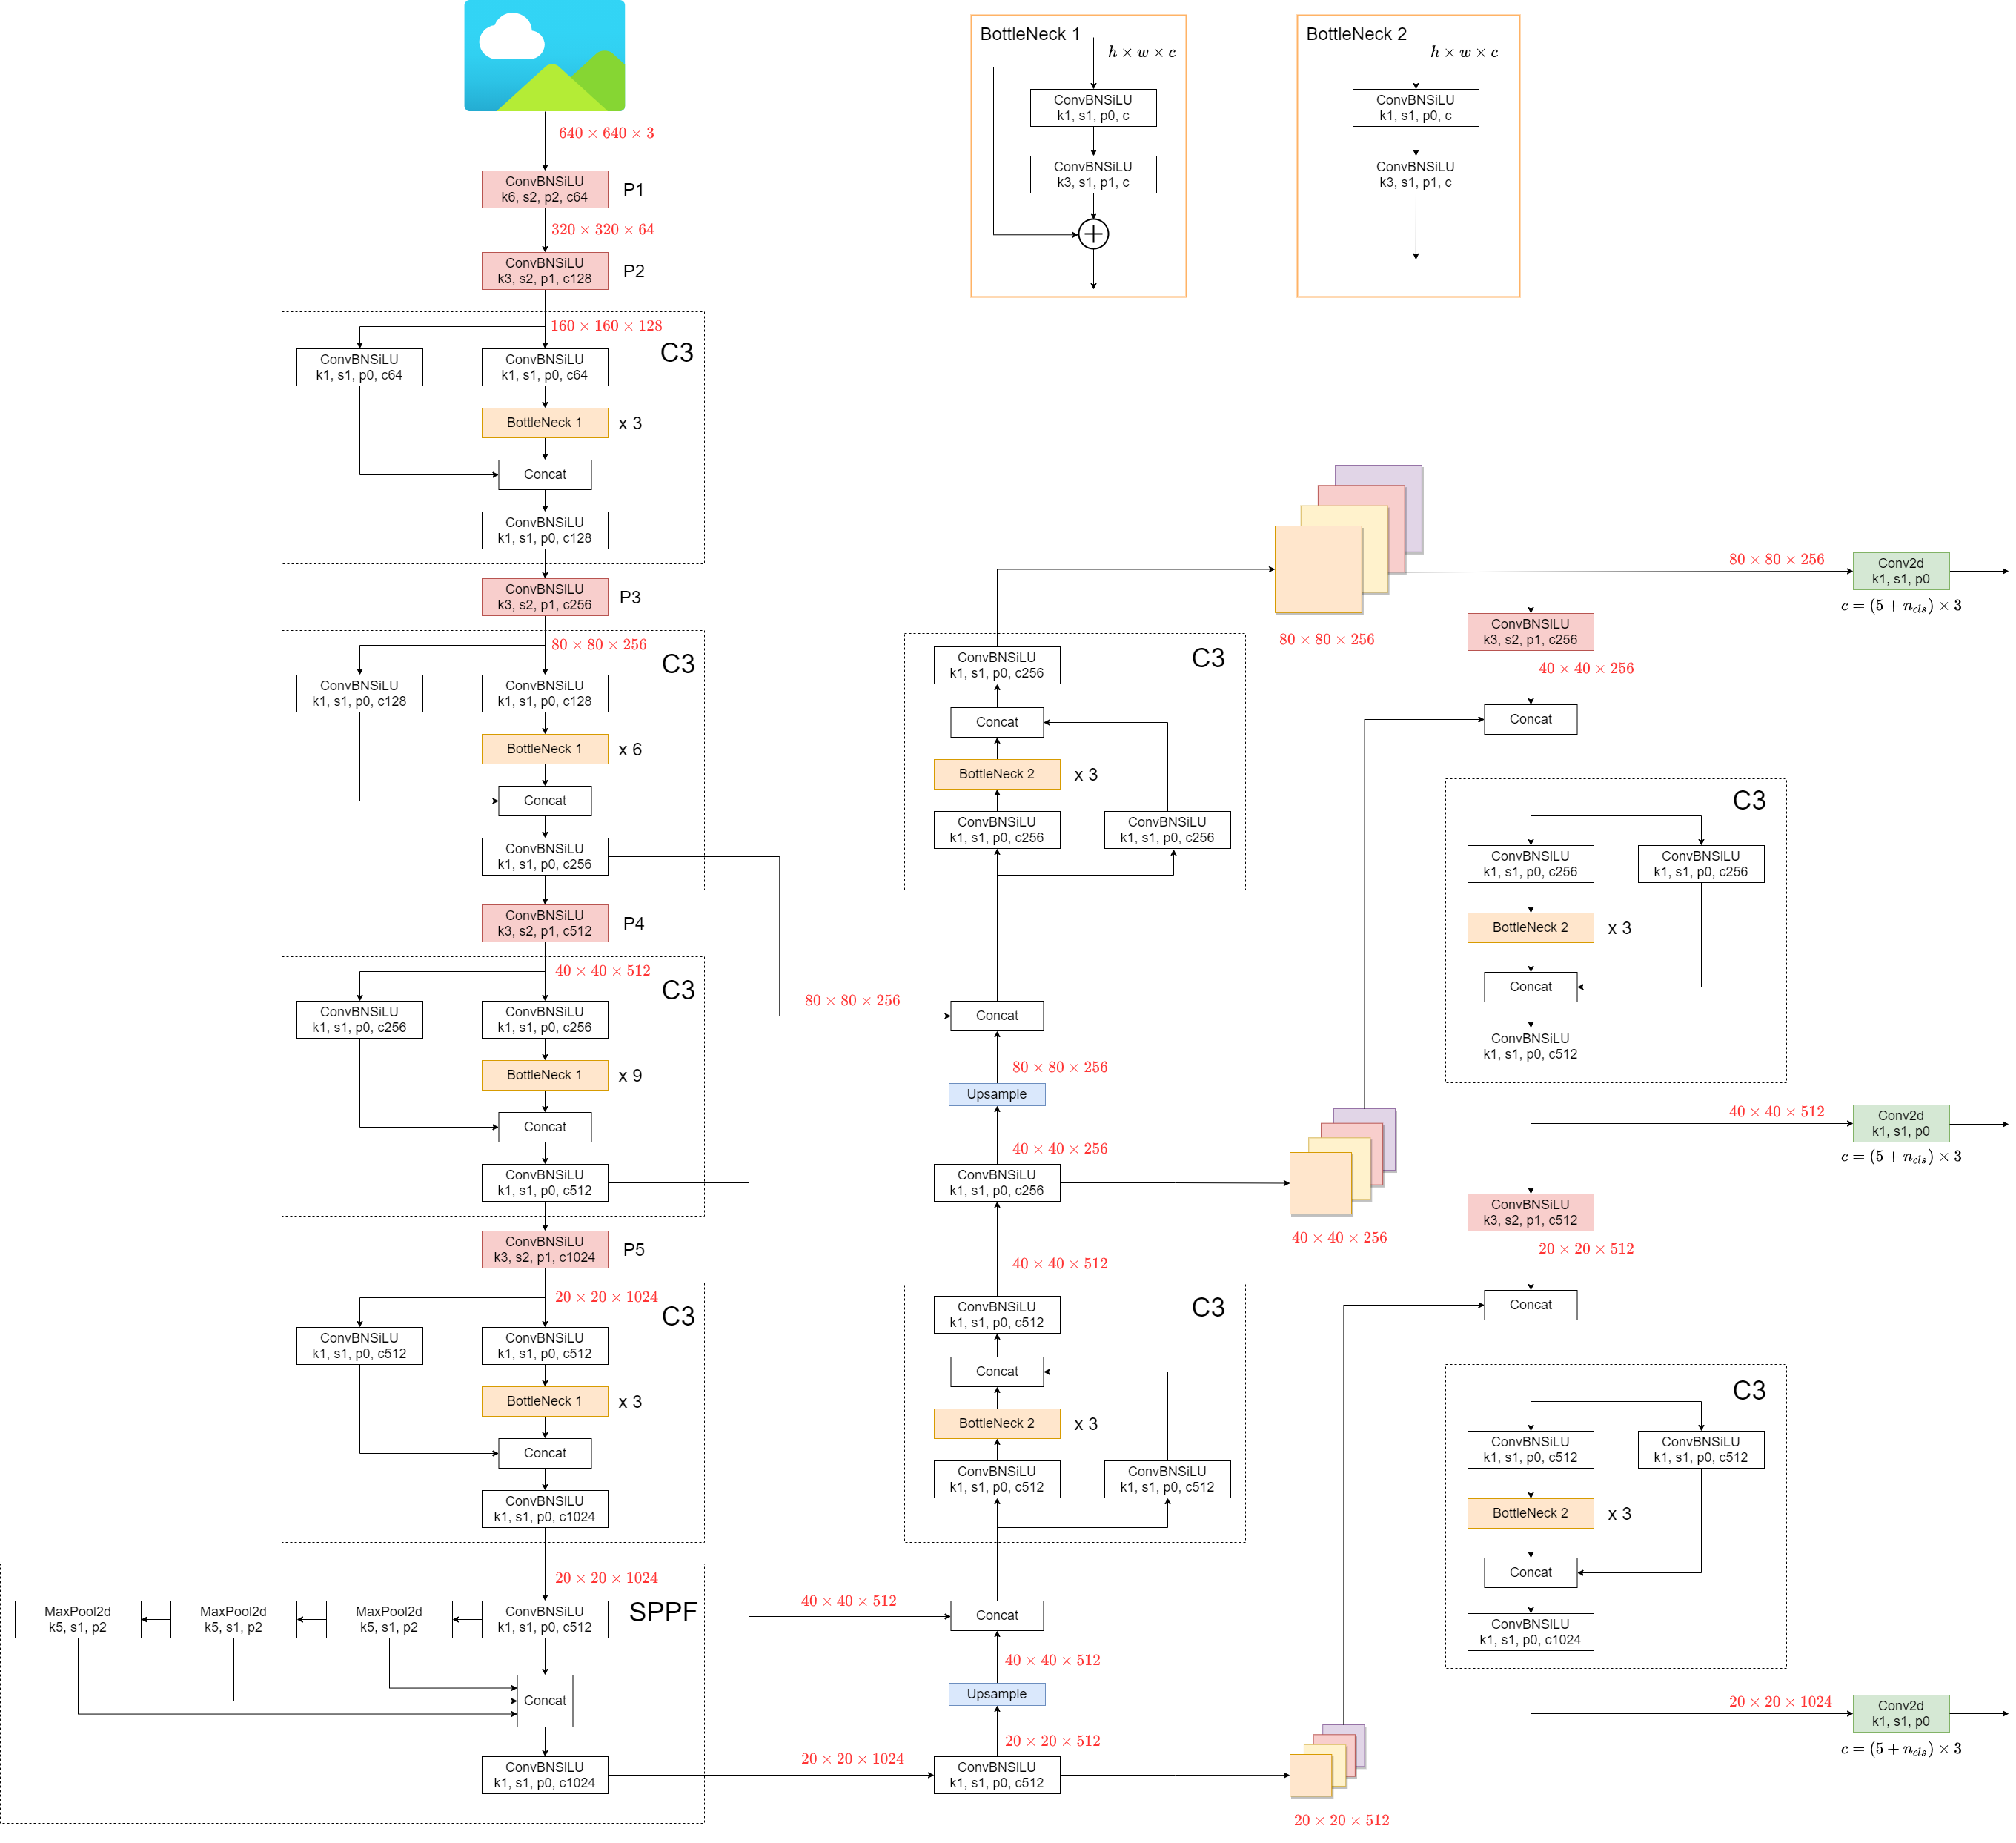
\includegraphics[width=1\textwidth]{Sistema de vision artificial/YOLO/arquitectura.png}
	\caption{Estructura de YOLOv5l}
	\label{chap:Sistema de visión artificial fig:Arquitectura YOLO}
\end{figure}